R-CNN系列算法是一个很庞大的算法簇,Ross Girshick发表\textit{Rich Feature Hierarchies for Accurate Object Detection and Semantic Segmentation}\cite{rcnn}一文以来衍生出非常多的算法。在此,只介绍与R-CNN关系最亲密的算法,他们的发展顺序如图\ref{rcnn-dev}
\begin{uscfigure}
	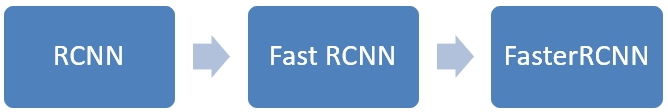
\includegraphics[width=\textwidth]{./Pictures/rcnn.jpg}	
	\caption{RCNN系列算法发展顺序}
	\label{rcnn-dev}
\end{uscfigure}

\par \noindent
他们在整个算法簇发展的过程中,更充分地利用Feature Maps的信息是系列算法发展的脉络。
\subsubsection{R-CNN}
RCNN:(Region CNN)\cite{rcnn}首次将深度学习应用到目标检测算法中。在PASCAL VOC\footnote{计算机视觉里面很大一块是在做物体的识别、检测还有分类(object recognition, detection and classification)。几乎在每一个应用领域都需要用到这三项功能,所以能否顺利的完成这三个功能,对检验一个算法的正确性和效率来说是至关重要的。所以每一个算法的设计者都会运用自己搜集到的场景图片对算法进行训练和检测,这个过程就逐渐的形成了数据集}的目标检测竞赛中,其作者Ross Girshick多次带领团队折桂。图\ref{rcnn}这个模型,“目标检测”领域内第一次结合了神经网络的结构图,其深远意义不言而喻。
\begin{uscfigure}
	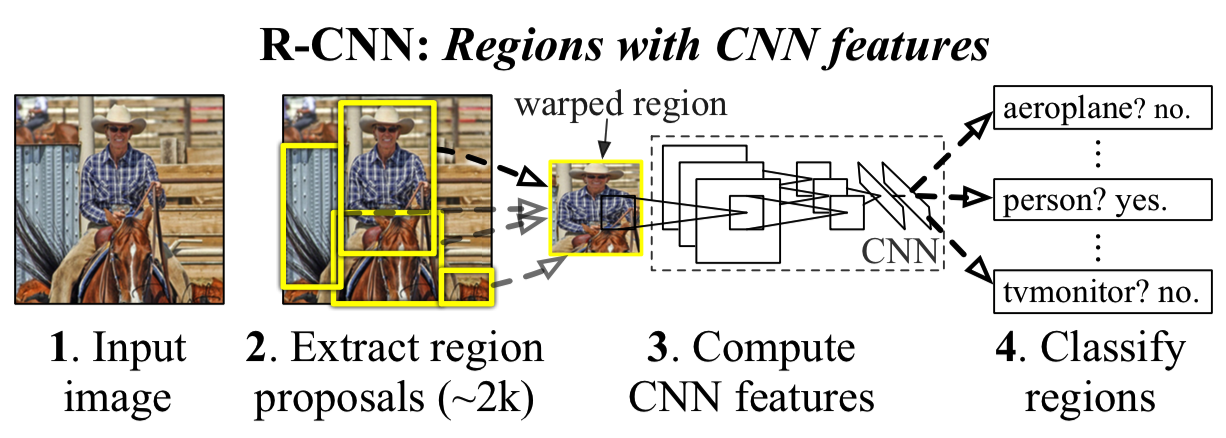
\includegraphics[width=\textwidth]{./Pictures/rcnn-regions_with_cnn_features.png}	
	\caption{RCNN算法框架}
	\label{rcnn}
\end{uscfigure}
该算法对目标检测中的两个关键问题提供了重要思路:

\textbf{解决问题一、速度。}
R-CNN使用启发式搜索方法(Selective Search\cite{ss})取代使用滑窗的区域选择算法。传统的区域选择算法,滑动一个窗口就需要检测一次,因此相邻窗口信息重叠高,导致检测速度慢。启发式搜索方法先生成候选区域再检测,大大降低了信息冗余的程度,从而检测速度得到提高。

\textbf{解决问题二、特征的鲁棒性。}
R-CNN使用卷积神经网络(CNN)提取特征取代人工设定的特征如Haar、HOG等。传统的手工提取特征鲁棒性差,特征设计复杂。仅限于低层次(Low-level)的特征如颜色、纹理等。使用CNN可以提取更高层面的抽象特征,从而提高特征的鲁棒性。

该方法将PASCAL VOC上的检测率从35.1\% 提高到53.7 \% 。

\textbf{算法流程:}

\line
\begin{itemize}
	\setlength{\itemsep}{0pt}
	\setlength{\parsep}{0pt}
	\setlength{\parskip}{0pt}
	\item[>] 一张图像生成1K至2K个候选区域;
	\item[>] 对每个候选区域,使用深度网络提取特征;
	\item[>] 特征送入每一类的SVM分类器,判别是否属于该类;
	\item[>] 使用回归器精细修正候选位置;
\end{itemize}
\line

\textbf{1、生成候选区域:}利用Selective Search\cite{ss}算法从原始图像中生成约2k-3k个候选区域。生成步骤:1、先将原始图像分割成小块区域。2、检索所有的小区域,合并最可能是属于同一个物体的两个区域。重复该操作直到整张图像中只剩下一个位置区域。3、输出所有候选的区域包括合并的区域,共同作为所谓的候选区域。

\textbf{2、提取特征:}利用2012年,Hinton在Image Net竞赛上提出的神经网络\footnote{Hinton在2012年提出的AlexNet网络}提取图像中的特征。

\textbf{3、判断类别:}对于每一类别的目标,使用线性SVM\cite{svm}分类器进行判别。输入为4096维特征向量,输出为此类别的置信度。同时原算法使用"Hard Negative Mining"\cite{hnm}方法。使正负样本的数量保持平衡。

\textbf{4、精修位置:}目标检测的结果好不好是看检测框与实际位置的重叠面积,故需要对检测的位置进行精修,以此提高检测精度。 

\subsubsection{SPP Net}
R-CNN提出后的一年,以何恺明、任少卿为首的团队发表了SPP Net:\textit{Spatial Pyramid Pooling in Deep Convolutional Networks for Visual Recognition}\cite{sppnet} ,这才是真正摸到了卷积神经网络的脉络。尽管R-CNN效果不错,但是他还有两个缺点:

\textbf{缺点一、算法过程冗余。}
R-CNN算法是先生成候选区域,再对该区域进行卷积,其导致的问题有二:其一是对相同区域进行了多次卷积,因为候选区域难免会有大量交叠的区域;其二是对存储空间浪费巨大,因为每个候选区域进行卷积后都需要新的存储空间。何恺明等人针对上述两点不足,交换了生成候选区域与卷积的顺序,通过巧妙地改变,不仅减少存储量而且大幅度地提高了训练速度。

\textbf{缺点二、图片缩放、裁剪问题。}
如图\ref{sppnet}所示,对于原始图片无论是缩放(Warp)还是裁剪(Crop),都会使原始图片的信息很大程度上的丢失从而影响训练效果。从示例图中可以看出,当把小车剪裁成一个车门,人们看到这个裁剪后的图片就难以判断图片的整体目标是一辆车;把一座高塔图片进行缩放后,也会使得机器的识别难度巨大。
\begin{uscfigure}
	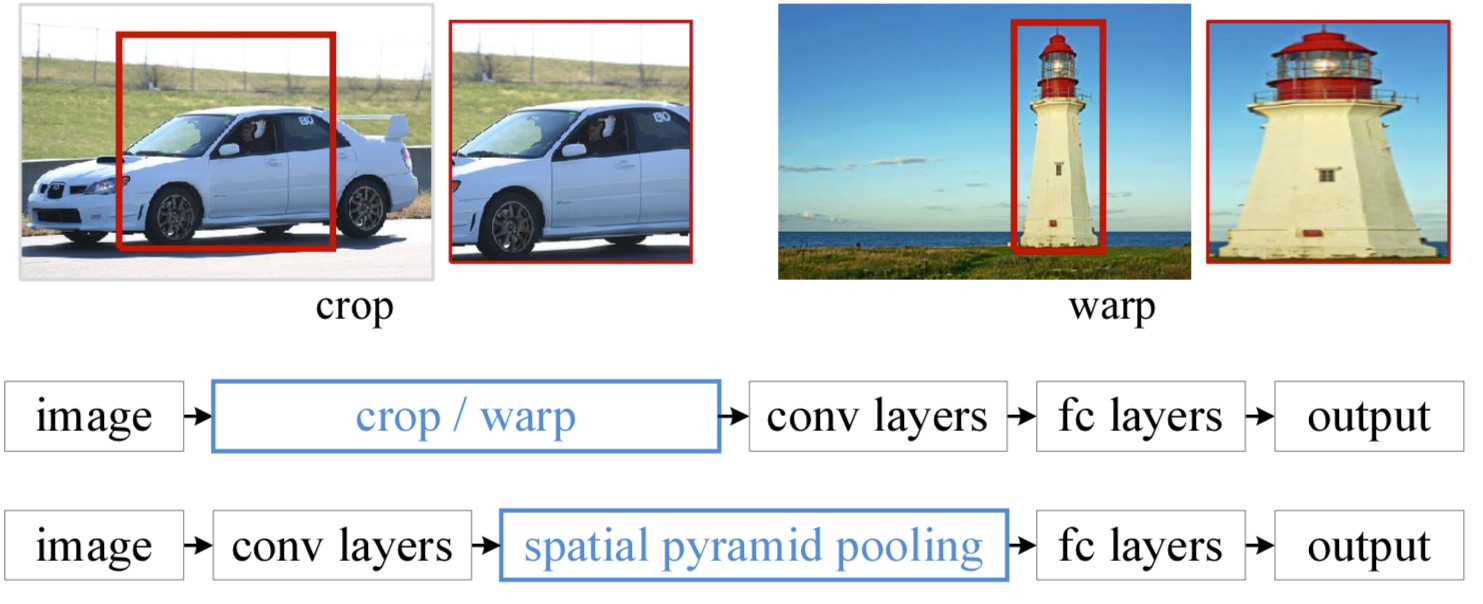
\includegraphics[width=\textwidth]{./Pictures/sppnet_crop_warp.jpg}	
	\caption{因剪裁和缩放导致视差}
	\label{sppnet}
\end{uscfigure}
问题的关键在于找到一个不对图片进行变形,且依然保留了原图整体信息的方法直接进行学习。最后,何恺明等人找到了问题的根源:全连接层(FC Layer)需要固定其输入向量维度,于是只需要定义一个特殊的池化层,使其输出的维度满足全连接层固定输入维度的要求即可。这个特殊的池化层将输入的任意尺度Feature Maps组合成特定维度的输出,如图\ref{sppnet},要输入的维度 $64∗256$ ,那么可以这样组合 $32∗256+16∗256+8∗256+8∗256$。
\begin{uscfigure}
	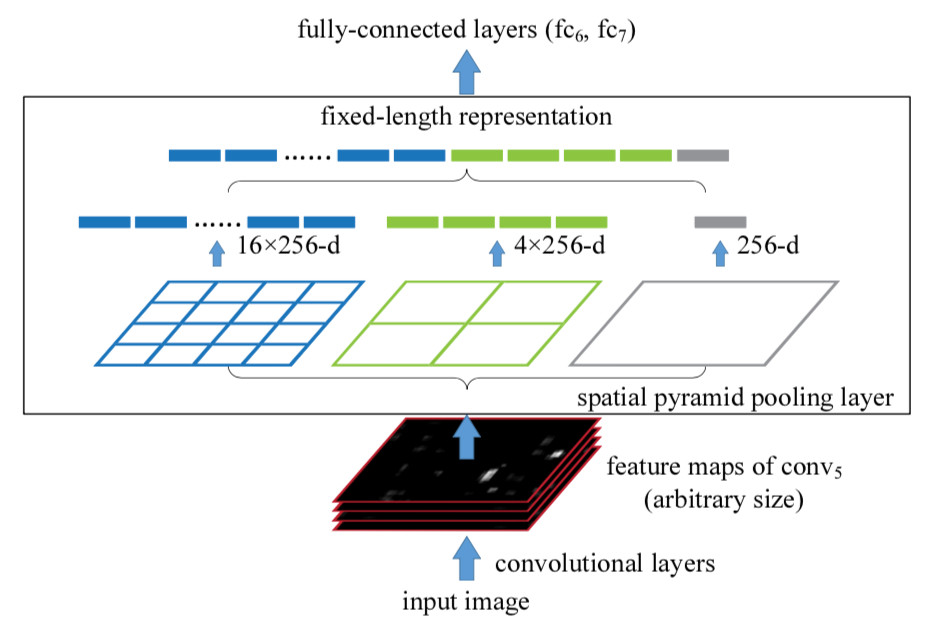
\includegraphics[width=\textwidth,]{./Pictures/sppnet_pool_layer.jpg}	
	\caption{输入维度的组合方式}
	\label{sppnet}
\end{uscfigure}
SPP Net的出现对整个目标检测及其相关领域产生了重要的影响,他不仅减少了计算冗余从而提高了检测速度,更重要的意义在于解禁了输入固定尺寸这一束缚,也因此被后面出现的算法广泛采用。本文基于的SSD算法就是更是从中受到启发。

\subsubsection{Fast R-CNN}
继2014年的RCNN之后,Ross Girshick在2015年发表了Fast RCNN\cite{fastrcnn},构思巧妙,算法流程更加紧凑,目标检测的速度也大幅提高。Fast R-CNN引用了SPP Net的贡献 。概括来说,贡献最大的地方在于用并行结构替换了原算法中的串行结构。Fast RCNN和RCNN相比,同样使用最大规模的网络,测试时间从47秒减少为0.32秒,训练时间从84小时减少为9.5小时。在PASCAL-VOC2007上的准确率,约在66\%-67\%之间。其算法框架如图\ref{fast-rcnn}
\begin{uscfigure}
	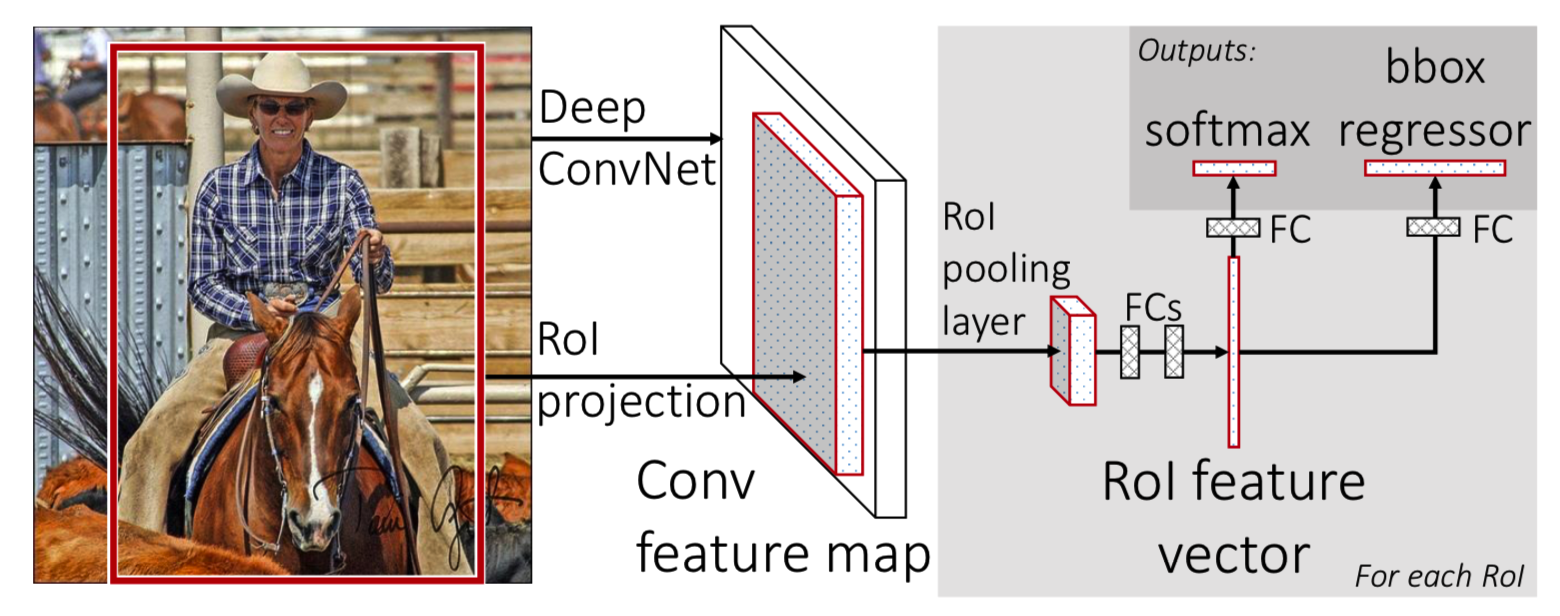
\includegraphics[width=\textwidth]{./Pictures/fast_rcnn.png}	
	\caption{Fast R-CNN算法框架}	
	\label{fast-rcnn}
\end{uscfigure}
R-CNN算法是先对候选框区域进行分类,如果检测到目标则对边界框(Bounding Box)进行精修、回归。全过程是串联的。能不能改成并联的呢?Ross Girshick将算法过程改成了并行结构——边分类,边对Bounding box进行回归。用一个Loss函数将conf-loss和loc-loss整合到了一起,同时也吸收了SPP Net算法的长处,因此其速度和精度都得到了提高。

\textbf{算法流程:}

\line
\begin{itemize}
	\setlength{\itemsep}{0pt}
	\setlength{\parsep}{0pt}
	\setlength{\parskip}{0pt}
	\item[>] 在图像中确定1000-2000个候选框 
	\item[>] 对于每个候选框内图像块,使用深度网络提取特征
	\item[>] 对候选框中提取出的特征,使用分类器判别是否属于一个特定类
	\item[>] 对于属于某一特征的候选框,用回归器进一步调整位置
\end{itemize}
\line\\
Fast RCNN算法针对RCNN算法中的三个方面进行了改进:

\textbf{第一个方面、测试时的速度慢。}由于RCNN算法中对一张图像内的候选框之间存在大量交叠部分,所以提取特征时的操作冗余,Fast R-CNN算法将整张归一化后的图像直接送入深度神经网络中。在与后面的网络邻接时,才将候选框的信息加入进来,从而共享了卷积操作,达到了提高速度的目的。

\textbf{第二个方面、训练时的速度慢。}其具体的原因同第一个方面,在训练时候,先将一张归一化后的图像送入深度神经网络中,紧接着将这幅图像上提取出的候选区域传入网络。所以避免了候选区域特征的重复计算。

\textbf{第三个方面、训练存储空间大。}RCNN算法中需要大量特征作为训练样本用来训练独立的分类器和回归器,Fast R-CNN不需要额外的存储,将类别判断和位置精修合并到一起,用一个统一的深度神经网络来实现。其网络模型如图\ref{fast-rcnn-model}

\begin{uscfigure}
	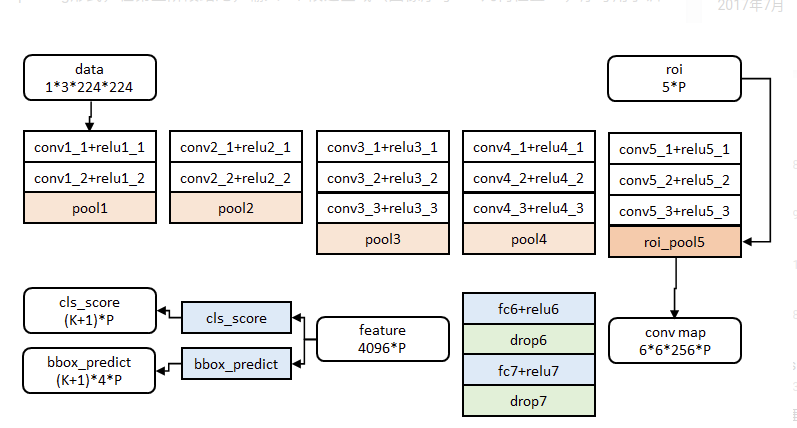
\includegraphics[width=\textwidth]{./Pictures/fast-rcnn-model.png}	
	\caption{Fast R-CNN网络模型}	
	\label{fast-rcnn-model}
\end{uscfigure}

\textbf{损失函数:}
loss\_cls评估分类损失。由其真实类别$u$对应的概率决定:
\begin{equation}
	L_{cls} = - \log p_u
\end{equation}
loss\_bbox评估检测框定位损失。由其真实类别对应的预测位置参数$t^u$和真实位置关于平移缩放$v$的因子来决定:
\begin{equation}
	L_{loc} = \sum_{i=1}^{4} g(t_i^u - v_i)
\end{equation}
	
g为Smooth L1误差,对outlier不敏感:
\begin{equation}
	g(x) = \left \{
		\begin{aligned}
		& 0.5x^2 	 & |x| < 1	\\	
		& |x| - 0.5  &otherwise
		\end{aligned}
		\right .
\end{equation}
如果分类为背景则不考虑定位代价,最后总的损失为二者加权和:
\begin{equation}
	L = \left \{
		\begin{aligned}
		& L_{cls} + \lambda L_{loc} & u\\
		& L_{cls} 					& u
		\end{aligned}
	\right .
\end{equation}
\subsubsection{Faster R-CNN}
继发表RCNN,Fast RCNN两篇力作之后,Ross Girshick等人又在2015年提出了Faster R-CNN\cite{fasterrcnn}算法。该算法在PASCAL VOC数据集上准确率为59.9\%,在简单网络目标上的检测速度达到17FPS;复杂网络目标上的检测准确率78.8\%,速度达到5FPS。在Faster R-CNN算法被提出前,所有的目标检测算法都是基于Low Level特征采用启发式搜索算法生产候选区域。这种策略存在着两个缺点:

\textbf{第一个缺点}候选区域具有不确定性。“Two Stage”系列算法为了解决这个问题生成了大量无效区域造成了大量多余的计算、可是如果减少了候选区域则又会使之漏检;

\textbf{第二个缺点}算法第一步——生成候选区域的算法是在CPU上运行的,与在GPU上训练的跨结构交互损失了算法效率。

于是乎,针对上述两个缺点,任少卿等人提出利用神经网络代替Selective Search算法自己去学习生成候选区域。将这个网络称之为RPN:Region Proposal Networks。其结构如图\ref{rpn}。
\begin{uscfigure}
	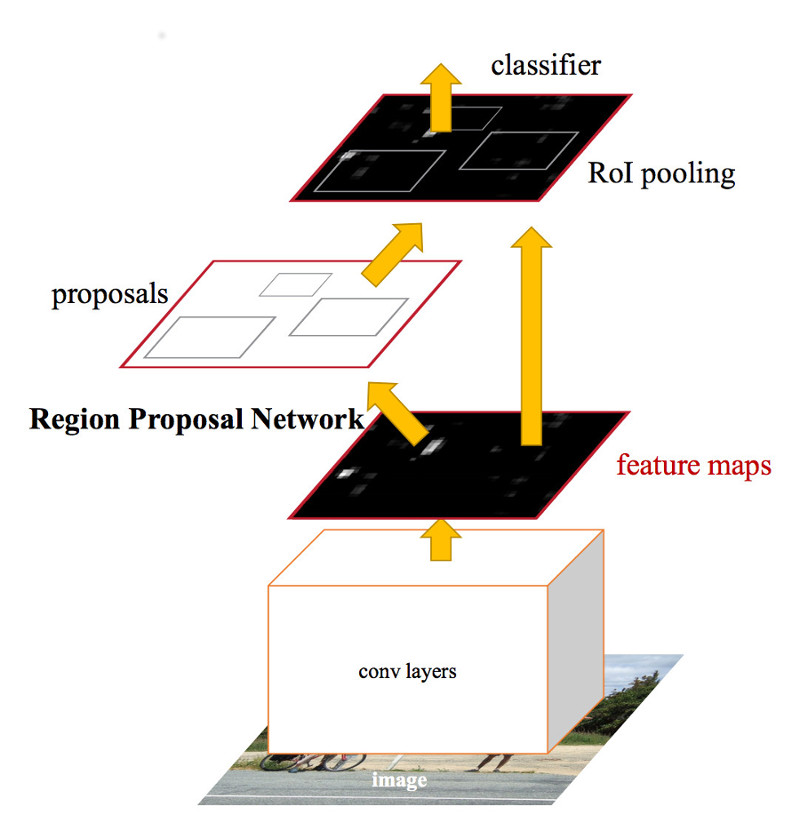
\includegraphics[width=\textwidth,height=8cm]{./Pictures/faster_rcnn.jpg}	
	\caption{Faster RCNN算法架构}	
	\label{rpn}
\end{uscfigure}
神经网络可以学到比Low Leval特征更加抽象、语义、高层的特征,同时大大提高了候选区域的可靠程度,利用RPN生成候选区域的方法一石二鸟,可以从图\ref{rpn}看出,将RPNs嵌入原有网络使RPNs和RoI Pooling层共用前面的卷积神经网络,整合原有网络和RPNs网络一起参与预测,参数量和预测时间都有在幅度的减少。值得一提的是,在RPN中引入了anchor的概念。对于Feature Map中的每个滑窗位置都会生成k个anchors,然后根据anchor与ground truth的IOU判断anchor覆盖的图像区域是前景还是背景,判断的同时回归Bounding box的精细位置。

Faster RCNN是RCNN系列算法中的集大成者,将目标检测算法的基本步骤\footnote{候选区域生成,特征提取,分类,位置精修}整合到了一个深度网络框架之内。其中所有计算共享,全部在GPU中完成,速度和精度都得到了极大的提高。

Faster RCNN始终围绕着三个问题展开:

\line
\begin{itemize}
	\setlength{\itemsep}{0pt}
	\setlength{\parsep}{0pt}
	\setlength{\parskip}{0pt}
	\item[>] 如何设计区域生成网络?
	\item[>] 如何训练区域生成网络?
	\item[>] 如何让区域生成网络和Faster RCNN网络共享特征提取网络?
\end{itemize}
\line

\textbf{区域生成网络(RPN)}

\textbf{1、特征提取:}如图\ref{rpn}灰色方框,是对原始特征提取(用任何分类模型进行提取都可)

\textbf{2、候选区域:}对于图像中的每一个位置,约定9个设定的候选窗口:三种不同比例{1:1,1:2,2:1}×三种不同面积{1282,2562,5122}。这些候选窗口被称之为anchors。如图\ref{anchor}示出51*39个anchor中心,以及9种anchor。
 
\begin{uscfigure}
	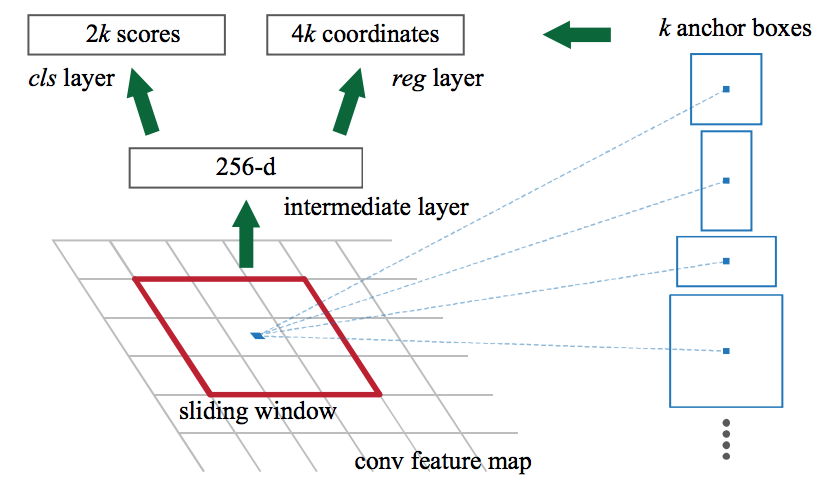
\includegraphics[width=\textwidth,height=8cm]{./Pictures/faster_rcnn_anchor.png}	
	\caption{Faster RCNN anchor示意图}	
	\label{anchor}
\end{uscfigure}

\textbf{3、位置精修和窗口分类:}分类层(cls\_score)计算每一个锚点上9个anchors属于前景和背景的概率;回归层(bbox\_pred)计算每一个锚点上9个anchors对应窗口平移缩放的参数。对于每个锚点输出$9*(4+1)$个参数



